\documentclass[a4paper, twocolumn]{article}
\usepackage[utf8]{inputenc}
\usepackage[T1]{fontenc}
\usepackage[pdftex, hidelinks,
            pdftitle={Real-Time Ocean Simulation and Rendering Using Gerstner Waves},
            pdfauthor={Erik Sven Vasconcelos Jansson},
            pdfsubject={Computer Graphics -- Procedural Animation},
            pdfkeywords={real-time,ocean,simulation,rendering,
                         opengl,glsl,gerstner,wave}]{hyperref}

\usepackage{bm}
\usepackage{caption}
\usepackage{listings}
\usepackage{pdfpages}
\usepackage{booktabs}
\usepackage{mathtools}
\usepackage{blindtext}
\usepackage{algorithmic}
\usepackage{graphicx}
\usepackage{courier}
\usepackage{acronym}
\usepackage{amssymb}
\usepackage{amsthm}
\usepackage{siunitx}
\usepackage{algorithm}
\usepackage[capitalize, noabbrev]{cleveref}
\usepackage[activate={true, nocompatibility}, final,
            tracking=true, kerning=true, spacing=true,
            factor=1100, stretch=10, shrink=10]{microtype}

\DeclareCaptionFormat{modifiedlst}{\rule{\linewidth}{0.85pt}\\[-2.9pt]#1#2#3}
\captionsetup[lstlisting]{format =  modifiedlst,
labelfont=bf,singlelinecheck=off,labelsep=space}
\lstset{basicstyle=\footnotesize\ttfamily,
        breakatwhitespace = false,
        breaklines = true,
        keepspaces = true,
        language = C++,
        showspaces = false,
        showstringspaces = false,
        frame = tb,
        numbers = left,
        numbersep = 5pt,
        xleftmargin = 16pt,
        framexleftmargin = 16pt,
        belowskip = \bigskipamount,
        aboveskip = \bigskipamount,
        escapeinside={<@}{@>}}

\title{\vspace{-1.5em}\textbf{Real-Time Ocean Simulation and \\
                              Rendering Using Gerstner Waves}}
\author{{\textbf{Erik Sven Vasconcelos Jansson}} \\
        {\href{mailto:erija578@student.liu.se}
        {\texttt{<erija578@student.liu.se>}}} \\
        {Linköping University, Sweden}}

\begin{document}

    \maketitle

    \begin{abstract} \blindtext
 \end{abstract}
    \begin{figure}[h]
        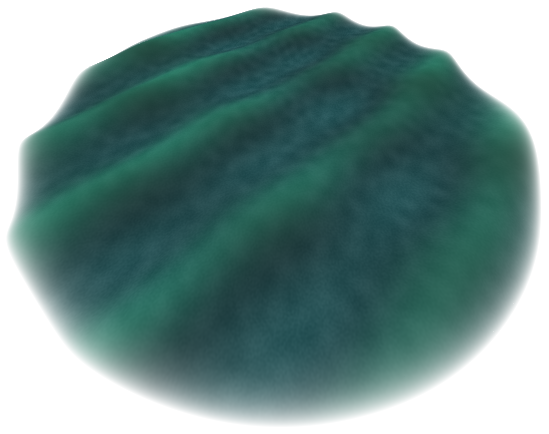
\includegraphics[width=\linewidth]{figures/gerstner.png}
    \end{figure} \newpage
    \section{Introduction} \label{sec:introduction} \Blindtext

    \section{Related Work} \label{sec:related_work} \begin{equation} \label{eq:sum_of_sine_waves}
    H(\mathbf{p},t) = \sum{
        A_i \sin \, (
            (\mathbf{p} \cdot \mathbf{d}_i) w_i
            + t \varphi_i
        )
    }
\end{equation}

\begin{equation} \label{eq:sum_of_sine_waves_position}
    \mathbf{H}(x,z,t) = \begin{bmatrix}
        x&
        H(\mathbf{p},t)&
        z
    \end{bmatrix}\;\,,\;\,
    \mathbf{p} = \begin{bmatrix}
        x&z
    \end{bmatrix}
\end{equation}

\begin{equation} \label{eq:sum_of_sine_waves_normal}
    \mathbf{\hat{H}}(x,z,t) = \begin{bmatrix}
        -\frac{\partial}{\partial x} H(\mathbf{p},t)&
        1&
        -\frac{\partial}{\partial z} H(\mathbf{p},t)
    \end{bmatrix}
\end{equation}

\begin{equation} \label{eq:gerstner_wave}
    G_j(\mathbf{p},t) = \sum{
        d_{i,j} Q_iA_i \cos \, (
            (\mathbf{p} \cdot \mathbf{d}_i) w_i
            + t \varphi_i
        )
    }
\end{equation}

\begin{equation} \label{eq:gerstner_wave_position}
    \mathbf{G}(x,z,t) = \begin{bmatrix}
        x + G_x(\mathbf{p},t)\\
        H(\mathbf{p},t)\\
        z + G_z(\mathbf{p},t)
    \end{bmatrix}\;\;\,,\;\;\,
    \mathbf{p} = \begin{bmatrix}
        x&z
    \end{bmatrix}
\end{equation}

\begin{equation} \label{eq:gerstner_wave_normal}
    \begin{split}
    \mathbf{\hat{G}}(x,z,t) &= \begin{bmatrix}
        -\sum{d_{i,x} A_iw_i \cos \psi_i}\\
        1 - \sum{Q_iA_iw_i \sin \psi_i}\\
        -\sum{d_{i,z} A_iw_i \cos \psi_i}
    \end{bmatrix}\;,\\
        \psi_i &= (\mathbf{G}(x,z,t) \cdot \mathbf{d}_i)w_i + t \varphi_i
    \end{split}
\end{equation}

    \section{Implementation} \label{sec:implementation} \Blindtext

\begin{lstlisting}[language=Python, caption=Python example]
import numpy as np

def incmatrix(genl1,genl2):
    m = len(genl1)
    n = len(genl2)
    M = None #to become the incidence matrix
    VT = np.zeros((n*m,1), int)  #dummy variable

    #compute the bitwise xor matrix
    M1 = bitxormatrix(genl1)
    M2 = np.triu(bitxormatrix(genl2),1) 

    for i in range(m-1):
        for j in range(i+1, m):
            [r,c] = np.where(M2 == M1[i,j])
            for k in range(len(r)):
                VT[(i)*n + r[k]] = 1;
                VT[(i)*n + c[k]] = 1;
                VT[(j)*n + r[k]] = 1;
                VT[(j)*n + c[k]] = 1;

                if M is None:
                    M = np.copy(VT)
                else:
                    M = np.concatenate((M, VT), 1)

                VT = np.zeros((n*m,1), int)

    return M
\end{lstlisting}

\Blindtext

    \section{Results} \label{sec:results} \Blindtext

\begin{figure}[t]
    \includegraphics[width=\linewidth]{example-image-b}
    \caption{Example figure}
\end{figure}

\Blindtext

\begin{table}[b]
    \centering
    \begin{tabular}{llr}
        \toprule
        \multicolumn{2}{c}{Item} \\
        \cmidrule(r){1-2}
        Animal    & Description & Price (\$) \\
        \midrule
        Gnat      & per gram    & 13.65      \\
            &    each     & 0.01       \\
        Gnu       & stuffed     & 92.50      \\
        Emu       & stuffed     & 33.33      \\
        Armadillo & frozen      & 8.99       \\
        \bottomrule
    \end{tabular}
    \caption{Some sort of data?}
\end{table}

    \section{Conclusions} \label{sec:conclusions} \blindtext[4]

\begin{equation}
    i\hbar\frac{\partial}{\partial t}\left|\Psi(t)\right>=H\left|\Psi(t)\right>
\end{equation}

\blindtext \cite{lamport1994latex}


    \newpage

    \section*{Acknowledgements}

    \nocite{*} % TODO: remove
    \bibliographystyle{abbrv}
    \bibliography{paper}

    \appendix
    \clearpage \onecolumn
    \lstinputlisting[caption={Gerstner Wave Shader for OpenGL with GLSL 4.10.},
                 morekeywords={vec2, vec3, uniform, uint, version, dot, sin, cos, inout},
                 label={lst:gerstner}]{listings/gerstner.glsl} \newpage
\lstinputlisting[caption={Tessellation Control Shader in GLSL 4.10 for Deciding the Ocean Surface Level-of-Detail.},
                 morekeywords={vec2, vec3, uniform, uint, version, dot, sin, cos, inout,
                               layout, vertices, in, out, distance, smoothstep, gl_InvocationID, gl_TessLevelInner, gl_TessLevelOuter},
                 label={lst:tesc}]{listings/gerstner.tesc} \newpage
\lstinputlisting[caption={Tessellation Evaluation Shader in GLSL 4.10 for Displacing Tessellated Ocean Surface.},
                 morekeywords={vec2, vec3, uniform, uint, version, dot, sin, cos, inout,
                               layout, in, out, distance, smoothstep,
                               quads, fractional_even_spacing, mix, vec4, gl_TessCoord, gl_Position},
                 label={lst:tese}]{listings/gerstner.tese} \newpage
\lstinputlisting[caption={Fragment Shader for Coloring the Ocean Surface (with a Fog Effect for Hiding Pop-in).},
                 morekeywords={vec2, vec3, uniform, uint, version, dot, sin, cos, inout,
                               in, out, smoothstep, mix, normalize, clamp, pow, distance, vec4, snoise3d},
                 label={lst:frag}]{listings/gerstner.frag} \newpage
\lstinputlisting[caption={Blinn--Phong Reflection Model Shader.},
                 morekeywords={vec2, vec3, uniform, uint, version, dot, sin, cos, inout,
                               in, out, smoothstep, mix, normalize, clamp, pow, distance, vec4, max, length},
                 label={lst:blinn_phong}]{listings/lighting.glsl} \newpage


\end{document}
